\section{DIL\_\-Hierarchy\_\-Level\_\-Data  Class Reference}
\label{classDIL__Hierarchy__Level__Data}\index{DIL_Hierarchy_Level_Data@{DIL\_\-Hierarchy\_\-Level\_\-Data}}
{\tt \#include $<$dil2al.hh$>$}

Inheritance diagram for DIL\_\-Hierarchy\_\-Level\_\-Data::\begin{figure}[H]
\begin{center}
\leavevmode
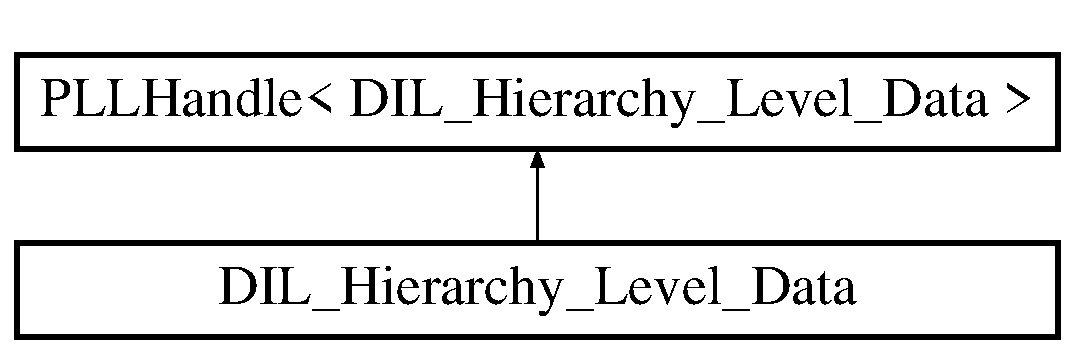
\includegraphics[height=2cm]{classDIL__Hierarchy__Level__Data}
\end{center}
\end{figure}
\subsection*{Public Methods}
\begin{CompactItemize}
\item 
{\bf DIL\_\-Hierarchy\_\-Level\_\-Data} ({\bf DIL\_\-entry} \&e, double l=DILSUPS\_\-REL\_\-UNSPECIFIED)
\item 
{\bf DIL\_\-entry} $\ast$ {\bf Entry} ()
\item 
virtual void {\bf reset\_\-benefit\_\-risk} ()
\item 
virtual bool {\bf has\_\-benefit\_\-risk} ()
\end{CompactItemize}
\subsection*{Public Attributes}
\begin{CompactItemize}
\item 
double {\bf likelihood}
\item 
double {\bf benefit}
\item 
double {\bf risk}
\end{CompactItemize}
\subsection*{Protected Attributes}
\begin{CompactItemize}
\item 
{\bf DIL\_\-entry} $\ast$ {\bf entry}
\end{CompactItemize}


\subsection{Constructor \& Destructor Documentation}
\index{DIL_Hierarchy_Level_Data@{DIL\_\-Hierarchy\_\-Level\_\-Data}!DIL_Hierarchy_Level_Data@{DIL\_\-Hierarchy\_\-Level\_\-Data}}
\index{DIL_Hierarchy_Level_Data@{DIL\_\-Hierarchy\_\-Level\_\-Data}!DIL_Hierarchy_Level_Data@{DIL\_\-Hierarchy\_\-Level\_\-Data}}
\subsubsection{\setlength{\rightskip}{0pt plus 5cm}DIL\_\-Hierarchy\_\-Level\_\-Data::DIL\_\-Hierarchy\_\-Level\_\-Data ({\bf DIL\_\-entry} \& {\em e}, double {\em l} = DILSUPS\_\-REL\_\-UNSPECIFIED)\hspace{0.3cm}{\tt  [inline]}}\label{classDIL__Hierarchy__Level__Data_a0}




Definition at line 730 of file dil2al.hh.

References benefit, DILSUPS\_\-REL\_\-UNSPECIFIED, likelihood, and risk.



\footnotesize\begin{verbatim}730 : entry(&e), likelihood(l), benefit(0.0), risk(0.0) {}
\end{verbatim}\normalsize 


\subsection{Member Function Documentation}
\index{DIL_Hierarchy_Level_Data@{DIL\_\-Hierarchy\_\-Level\_\-Data}!Entry@{Entry}}
\index{Entry@{Entry}!DIL_Hierarchy_Level_Data@{DIL\_\-Hierarchy\_\-Level\_\-Data}}
\subsubsection{\setlength{\rightskip}{0pt plus 5cm}{\bf DIL\_\-entry}$\ast$ DIL\_\-Hierarchy\_\-Level\_\-Data::Entry ()\hspace{0.3cm}{\tt  [inline]}}\label{classDIL__Hierarchy__Level__Data_a1}




Definition at line 734 of file dil2al.hh.

Referenced by DIL\_\-Visualize\_\-with\_\-FORM\_\-Tabs::Visualize\_\-Plan\_\-Entry().



\footnotesize\begin{verbatim}734 { return entry; }
\end{verbatim}\normalsize 
\index{DIL_Hierarchy_Level_Data@{DIL\_\-Hierarchy\_\-Level\_\-Data}!has_benefit_risk@{has\_\-benefit\_\-risk}}
\index{has_benefit_risk@{has\_\-benefit\_\-risk}!DIL_Hierarchy_Level_Data@{DIL\_\-Hierarchy\_\-Level\_\-Data}}
\subsubsection{\setlength{\rightskip}{0pt plus 5cm}virtual bool DIL\_\-Hierarchy\_\-Level\_\-Data::has\_\-benefit\_\-risk ()\hspace{0.3cm}{\tt  [inline, virtual]}}\label{classDIL__Hierarchy__Level__Data_a3}




Definition at line 736 of file dil2al.hh.

References benefit, and risk.

Referenced by DIL\_\-Visualize\_\-with\_\-FORM\_\-Tabs::Visualize\_\-Not\-Shown().



\footnotesize\begin{verbatim}736 { return ((benefit!=0.0) || (risk!=0.0)); }
\end{verbatim}\normalsize 
\index{DIL_Hierarchy_Level_Data@{DIL\_\-Hierarchy\_\-Level\_\-Data}!reset_benefit_risk@{reset\_\-benefit\_\-risk}}
\index{reset_benefit_risk@{reset\_\-benefit\_\-risk}!DIL_Hierarchy_Level_Data@{DIL\_\-Hierarchy\_\-Level\_\-Data}}
\subsubsection{\setlength{\rightskip}{0pt plus 5cm}virtual void DIL\_\-Hierarchy\_\-Level\_\-Data::reset\_\-benefit\_\-risk ()\hspace{0.3cm}{\tt  [inline, virtual]}}\label{classDIL__Hierarchy__Level__Data_a2}




Definition at line 735 of file dil2al.hh.

References benefit, and risk.



\footnotesize\begin{verbatim}735 { benefit=0.0; risk=0.0; }
\end{verbatim}\normalsize 


\subsection{Member Data Documentation}
\index{DIL_Hierarchy_Level_Data@{DIL\_\-Hierarchy\_\-Level\_\-Data}!benefit@{benefit}}
\index{benefit@{benefit}!DIL_Hierarchy_Level_Data@{DIL\_\-Hierarchy\_\-Level\_\-Data}}
\subsubsection{\setlength{\rightskip}{0pt plus 5cm}double DIL\_\-Hierarchy\_\-Level\_\-Data::benefit}\label{classDIL__Hierarchy__Level__Data_m1}




Definition at line 732 of file dil2al.hh.

Referenced by DIL\_\-Hierarchy\_\-Level\_\-Data(), has\_\-benefit\_\-risk(), reset\_\-benefit\_\-risk(), and DIL\_\-Visualize\_\-with\_\-FORM\_\-Tabs::Visualize\_\-Plan\_\-Entry().\index{DIL_Hierarchy_Level_Data@{DIL\_\-Hierarchy\_\-Level\_\-Data}!entry@{entry}}
\index{entry@{entry}!DIL_Hierarchy_Level_Data@{DIL\_\-Hierarchy\_\-Level\_\-Data}}
\subsubsection{\setlength{\rightskip}{0pt plus 5cm}{\bf DIL\_\-entry}$\ast$ DIL\_\-Hierarchy\_\-Level\_\-Data::entry\hspace{0.3cm}{\tt  [protected]}}\label{classDIL__Hierarchy__Level__Data_n0}




Definition at line 728 of file dil2al.hh.\index{DIL_Hierarchy_Level_Data@{DIL\_\-Hierarchy\_\-Level\_\-Data}!likelihood@{likelihood}}
\index{likelihood@{likelihood}!DIL_Hierarchy_Level_Data@{DIL\_\-Hierarchy\_\-Level\_\-Data}}
\subsubsection{\setlength{\rightskip}{0pt plus 5cm}double DIL\_\-Hierarchy\_\-Level\_\-Data::likelihood}\label{classDIL__Hierarchy__Level__Data_m0}




Definition at line 731 of file dil2al.hh.

Referenced by DIL\_\-Hierarchy\_\-Level\_\-Data(), and DIL\_\-Visualize\_\-with\_\-FORM\_\-Tabs::Visualize\_\-Plan\_\-Entry().\index{DIL_Hierarchy_Level_Data@{DIL\_\-Hierarchy\_\-Level\_\-Data}!risk@{risk}}
\index{risk@{risk}!DIL_Hierarchy_Level_Data@{DIL\_\-Hierarchy\_\-Level\_\-Data}}
\subsubsection{\setlength{\rightskip}{0pt plus 5cm}double DIL\_\-Hierarchy\_\-Level\_\-Data::risk}\label{classDIL__Hierarchy__Level__Data_m2}




Definition at line 733 of file dil2al.hh.

Referenced by DIL\_\-Hierarchy\_\-Level\_\-Data(), has\_\-benefit\_\-risk(), reset\_\-benefit\_\-risk(), and DIL\_\-Visualize\_\-with\_\-FORM\_\-Tabs::Visualize\_\-Plan\_\-Entry().

The documentation for this class was generated from the following file:\begin{CompactItemize}
\item 
{\bf dil2al.hh}\end{CompactItemize}
